\documentclass[a4paper, 14pt]{article}
\usepackage{float}
\usepackage{extsizes}
\usepackage{amsmath}
\usepackage{amssymb}
\everymath{\displaystyle}
\usepackage{geometry}
\usepackage{fancyhdr}
\usepackage{multicol}
\usepackage{graphicx}
\usepackage[brazil]{babel}
\usepackage[shortlabels]{enumitem}
\usepackage{cancel}
\columnsep=2cm
\hoffset=0cm
\textwidth=8cm
\setlength{\columnseprule}{.1pt}
\setlength{\columnsep}{2cm}
\renewcommand{\headrulewidth}{0pt}
\geometry{top=1in, bottom=1in, left=0.7in, right=0.5in}

\pagestyle{fancy}
\fancyhf{}
\fancyfoot[C]{\thepage}

\begin{document}
	
	\noindent\textbf{1EMMA03, 1EMMA04~Matemática} 
	
	\begin{center}Ângulos e polígonos no Tangram e resolução de problemas (Versão estudante)
	\end{center}
	
	\noindent\textbf{Nome:} \underline{\hspace{10cm}}
	\noindent\textbf{Data:} \underline{\hspace{4cm}}
	
	%\section*{Questões de Matemática}
	~ \\
	\indent Vamos iniciar esta sequência de atividades de forma mais interativa, através de um quebra-cabeça muito conhecido, formado por triângulos e quadriláteros 
	Você já ouviu falar no tangram? 
	O Tangram é um antigo jogo de quebra-cabeças chinês, que consiste na formação de figuras e desenhos por meio de 7 peças. 
\\
	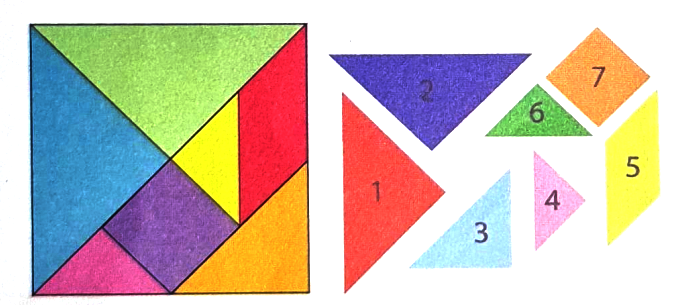
\includegraphics[width=1\linewidth]{1EMMA03_imagens/imagem01}
	
	\indent As regras desse jogo consistem em usar as sete peças em qualquer montagem colocando-as lado a lado sem sobreposição, com as quais é possível criar e montar cerca de 1700 figuras, como animais, pessoas, objetos, letras, números, figuras geométricas entre outros.
	\begin{enumerate}
		\item Vamos conhecer melhor as peças do Tangram? 
\\\\
		O Tangram é formado por cinco triângulos (2 grandes, 1 médio e 2 pequenos), 1 quadrado e 1 paralelogramo. \\
		Quais as medidas dos ângulos internos de cada peça? \\\\
		O Tangram é formado por cinco triângulos (2 grandes, 1 médio e 2 pequenos), 1 quadrado e 1 paralelogramo. \\
		Quais as medidas dos ângulos internos de cada peça? 
\\\\
		Triângulo grande:
\\\\\\
		Triângulo médio: 
\\\\\\
		Triângulo pequeno: 
\\\\\\
		Quadrado: 
\\\\\\
		Paralelogramo: 
\\\\\\
		\\
		\item Forme quadrados utilizando: 
\\
		a) 2 peças
~~~~~
		b) 3 peças
~~~~~
		c) 4 peças
~~~~~
		d) 5 peças
~~~~~
		\\\\\\\\\\\\\\\\
		\item Forme quadrados utilizando: 
\\
		a) 2 peças
~~~~~
		b) 3 peças
~~~~~
		c) 4 peças
~~~~~
		d) 5 peças
~~~~~
    \end{enumerate}
\end{document}